\section{Evaluation}\label{sec:eval}

\subsection{Experimental Setup}

\textbf{Frontends}

\begin{enumerate}

	\item AWS Step Functions

	\item (GCC workflows, which are Apache Airflow DAGs)

	\item PyWren code / mu (excamera) code

\end{enumerate}

\textbf{Backends}

\begin{enumerate}

	\item AWS Lambda + [s3, dynamodb, elasticache/redis]

	\item (Azure Functions + [])

	\item Google Cloud

\end{enumerate}

\textbf{Application Suite}

\begin{enumerate}
	\item All examples in the Step Function repository
	\item (GCC DAG repository)
	\item ExCamera
	\item IoT pipeline (chain)
	\item Word count (fan-out)
	\item Image processing (fan-out)
	\item (Hello Retail)
\end{enumerate}


\subsection{Capability/Expressiveness}

\name{}'s fundamental building blocks are much simpler than existing
systems. Can unum be as capable/expressive?

\name{} IR's expressiveness is what's really evaluated here. If there's a
category of workflows that our continuation-passing style IR cannot express,
that's a significant limitation.

\begin{itemize}

	\item Support 3 different types of frontends:

	\begin{enumerate}
		\item State machine: AWS Step Functions
		\item DAG: Google Cloud Composer (which is Apache Airflow)
		\item Procedural code DSL: mu/excamera or PyWren (both are limited and
		much less general than Durable Functions) or gg (gg has its own suite
		of applications)
	\end{enumerate}

	\item Take the full set of available applications in Step Functions,
(GCC), excamera, and show that unum can transform them into the IR and execute
on AWS. Publish the examples.

	\item Show that excamera cannot be efficiently expressed with Step
	Functions but can with unum.

\end{itemize}


\subsection{Runtime Overhead}

\name{} replaces workflow execution systems with a library that runs on
component functions. We should evaluate how much overhead the \name{} library
adds and how much extra costs in dollars they equate to.

\begin{itemize}
	\item Average additional latency as a percentage of average function
	runtime
	\item Latency for checkpointing (writing to data store)
	\item Latency for fan-in (reading multiple items from data store)
	\item Latency for invoking continuation
	\item Average additional memory consumption
	\item How much additional costs in dollars (both latency and memory) given
	average function size
\end{itemize}

\begin{figure}[t!]
    \centering
    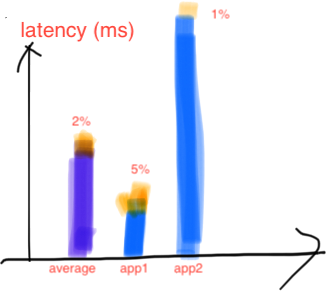
\includegraphics[width=\columnwidth]{figures/Sketch1.png}
    \caption{\name{} runtime latency overhead on average and for each workflow}
\end{figure}

\subsection{Performance}

\subsubsection{E2E Latency comparison against Step Functions (and
other orchestrators)}

Claim: (1). orchestration is distributed and automatically parallelized, (2).
Data only flow through the function that requires it, which reduces the amount
of network communication.

Hypothesis: \name{} is always faster than Step Functions, esp. for
highly-parallel applications (We saw very good preliminary results with the
parallel pipeline application).

\textbf{Experiment}: Keep a fixed request rate at a low level. Measure how
long it takes to complete a workflow invocation e2e.

Measurements should be done with both microbenchmarks and real applications.

\textbf{Microbenchmarks:}

It doesn't really matter what the user functions do. For the workflow system,
what we care about is function runtime, and orchestration pattern.
Microbenmarks allows us to control those factors and test the performance of
the workflow system.

Workflow patterns:

\begin{enumerate}
	\item Chains of various lengths
	\item Fan-out with different sizes (level of parallelism)
	\item Fan-out to chains of various lengths
\end{enumerate}

\textbf{Applications}

We should at least test

\begin{enumerate}
	\item ExCamera
	\item IoT pipeline (chain)
	\item Word count (fan-out)
	\item Image processing (fan-out)
\end{enumerate}

For ExCamera and word count, we should choose a high level of parallelism. For
example, 1000 mappers and reducers.

Note on throughput: We can't really measure throughput because we can't
saturate Lambda.

\begin{figure}[t!]
    \centering
    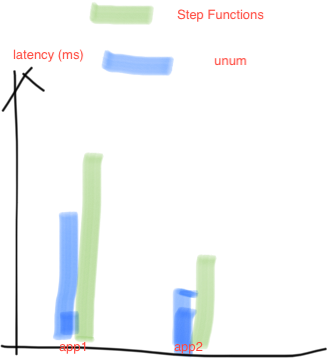
\includegraphics[width=\columnwidth]{figures/Sketch2.png}
    \caption{End-to-end latency for each workflow, \name{} vs Step Functions}
\end{figure}

\begin{figure}[t!]
    \centering
    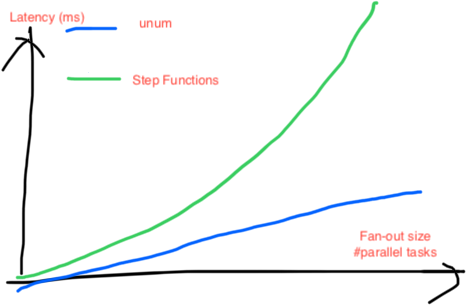
\includegraphics[width=\columnwidth]{figures/Sketch3.png}
    \caption{End-to-end latency for word count/excamera/parallel pipeline,
    \name{} vs Step Functions}
\end{figure}

\subsection{Pricing Comparison}

Dollar costs for programmers running the same workflow with \name{} vs Step
Functions.

Pick a few representative applications and show their results in a table.

\begin{enumerate}
	\item ExCamera
	\item IoT pipeline (chain)
	\item Word count (fan-out)
	\item Image processing (fan-out)
\end{enumerate}

\subsubsection{(Different Data Stores)}

To support the argument that \name{} can scale with the data store. Compare
E2E latency with different storage.
